\section{Les nombreux défis de l'annotation}
\label{section:2.3-DEFIS-ANNOTATION}

	%%%
	%%% Introduction: annoncer la complexité due (1) aux données (2) à la tâche et (3) aux humains.
	%%%
	
	Comme nous avons pu l'apercevoir dans les sections précédentes, le cycle d'annotation recèle de zones d'ombres pouvant introduire des complications dans la conception d'une base d'apprentissage (\cite{baledent:2022:complexite-annotation-manuelle}).
	Pour aborder cette partie, nous alors voir :
	\begin{itemize}
		\item qu'il y a une forte pression sur la \textbf{qualité des données} devant constituer le corpus d'entraînement (cf. \textsc{Section~\ref{section:2.3.1-DEFIS-ANNOTATION-ASPECT-DONNEES}}) ;
		\item que ce standard de qualité entretient une \textbf{complexité inhérente} aux étapes de modélisation et d'annotation (cf. \textsc{Section~\ref{section:2.3.2-DEFIS-ANNOTATION-ASPECT-COMPLEXITE}}) ;
		\item et que cette complexité provoque des \textbf{différences de comportements} chez les annotateurs (cf. \textsc{Section~\ref{section:2.3.3-DEFIS-ANNOTATION-ASPECT-HUMAIN}}).
	\end{itemize}
	En détaillant chacun de ces trois points, nous discuterons de l'ensemble de techniques et bonnes pratiques mises en avant dans la littérature pour limiter les désagréments d'un projet d'annotation.
	Nous identifierons aussi les freins récurant pouvant intervenir dans les mises en application industrielles.
	
	
	%%%
	%%% Subsection 2.3.1: Défis concernant le besoin de qualité des données.
	%%%
	\subsection{Défis concernant le besoin de qualité des données}
	\label{section:2.3.1-DEFIS-ANNOTATION-ASPECT-DONNEES}
	
		% Introduction: Machine Learning = reproduire par l'exemple.
		Comme nous l'avons défini en \textsc{Section\ref{section:2.1.1.A-PRESENTATION-ANNOTATION-DEFINITION-MACHINE-LEARNING}}, l'\textguillemets{\texttt{apprentissage automatique}} regroupe un ensemble de techniques dont l'objectif est de reproduire une tâche \textbf{par l'exemple} : il est donc normal de porter une attention particulière aux données utilisées, car la qualité du modèle de \textit{Machine Learning} va fortement dépendre de la qualité de sa base d'apprentissage.
		Nous allons ici détailler trois défis actuels concernant cette création d'un jeu de données.
		
		
		%%% 2.3.1.A. Problèmes de représentativité.
		\subsubsection{Problèmes de représentativité}
		\label{section:2.3.1.A-DEFIS-ANNOTATION-ASPECT-DONNEES-REPRESENTATIVITE}
			
			% Introduction : Une collecte doit être "représentative" du problème.
			La phase de collecte de données est une étape importante du projet d'annotation.
			Malheureusement, la littérature scientifique associée à cette tâche est assez légère alors que c'est précisément à ce moment que ce joue une caractéristique cruciale de la future base d'apprentissage : la \textbf{représentativité} du phénomène à modéliser.
			
			% Définir la représentativité à partir de la méthode de l'échantillon.
			Cette notion est assez ambiguë, notamment car le terme technique \textguillemets{représentatif}fait écho à un mot de la vie courante qui peut avoir plusieurs sens.
			Dans \cite{kruskal-mosteller:1979:representative-sampling-nonscientific} et \cite{clemmensen-kjaersgaard:2022:data-representativity-machine}, plusieurs usages communs de ce terme sont recensés :
			\begin{itemize}
				\item \textguillemets{\textit{assertive claim}} :
				l'opérateur déclare que ses données sont représentatives du problème sans apporter d'arguments. Bien entendu, cette option est à bannir car elle n'apporte aucune information et peut cacher des vices de conception du modèle ;
				\item \textguillemets{\textit{absence or presence of selective force}} :
				la représentativité du phénomène est supposée en sélectionnant des données de \textbf{manière aléatoire} et en limitant le nombre de critères de sélection à ceux nécessaires pour l'étude réalisée ; 
				\item \textguillemets{\textit{miniature}} :
				aussi appelée \textbf{sélection stratifiée}, cette approche consiste à dire qu'un échantillon est représentatif d'un phénomène si la proportion de chacune de ses parties y est respectée
				(\textit{par exemple, un sondage peut respecter la répartition des tranches d'âge d'une population}) ;
				\item \textguillemets{\textit{typical/ideal case}} :
				cette définition consiste à représenter chaque partie du phénomène par un \textbf{exemple emblématique} ou un \textbf{exemple moyen}
				(\textit{par exemple, on peut illustrer l'univers de la bande dessinée française par un numéro de la saga \texttt{Astérix \& Obélix}}) ;
				\item \textguillemets{\textit{population coverage}} :
				ici, la représentativité est associée à la présence \textbf{exhaustive} de l'ensemble des caractéristiques importantes du phénomène avec au moins un exemple par caractéristique
				(\textit{par exemple, dans l'arche de Noé, il y devait y avoir au moins un couple de chaque animaux}).
			\end{itemize}
			
			% Définir la représentativité à partir de la méthode d'échantillonnage.
			Pour compléter ces définitions, \cite{kruskal-mosteller:1979:representative-sampling-ii} incitent sur le besoin de \textbf{définir avec précision la méthode d'\textit{échantillonnage}} plutôt que l'\textit{échantillon} lui-même : en effet, il est important de caractériser le phénomène à modéliser, de définir l'objectif de la collecte de données et de détailler comment cette collecte va être réalisée.
			\cite{clemmensen-kjaersgaard:2022:data-representativity-machine} introduisent à leur tour trois mesures pour aider à caractériser une collecte : la \textit{réflexion} (est-ce l'échantillon respecte la distribution de la population ?), la \textit{couverture} (est-ce que l'échantillon illustre la diversité de la population ?) et la \textit{présence de représentants} (est-ce que l'échantillon contient les exemples emblématiques de la population ?).
			De telles informations sont essentielles pour pouvoir juger de la valeur d'un échantillon par rapport à un cas d'usage et déterminer s'il est réutilisable dans pour une autre application.
			%
			\begin{leftBarExamples}
				% Cas d'usage : classification d'état.
				Illustrons nos propos avec la classification de l'état d'une bande dessinée à partir d'une photo (voir \textsc{Section~\ref{section:2.1.2.B-PRESENTATION-ANNOTATION-EXEMPLES-CLASSIFICATION}}).
				Afin de représenter correctement le cas d'usage, nous pourrions collecter des exemples de \texttt{BD} couvrant l'ensemble des dégradations fréquemment identifiées par les libraires (couvertures froissées, pages déchirées, couleurs délavées, ...) et les intégrer de manière proportionnelle dans la base d'apprentissage.
				Nous pourrions aussi nous assurer de la présence de cas emblématiques permettant de catégoriser les \texttt{BD} en "\texttt{Mauvais état}", "\texttt{Bon état}", "\texttt{Très bon état}", "\texttt{Neuf}".
				
				% Autre cas d'usage : pas représentatif.
				Toutefois, cette base d'apprentissage ne sera plus représentative si nous voulons détecter la langue de la bande dessinée (auquel cas, une répartition par langue sera a priori plus adéquate).
			\end{leftBarExamples}
			
			% Besoin de beaucoup d'exemples.
			La description d'un phénomène reste cependant une \textbf{tâche difficile}, notamment lorsque que celui-ci possède un ensemble vaste et abstrait de caractéristiques à décrire.
			Nous comptons généralement sur la loi des grands nombres pour espérer dresser un portrait fidèle du phénomène, mais cela impose parfois de traiter des \textbf{immenses quantités de données}.
			%
			\begin{leftBarExamples}
				% Exemple de la variabilité du langage.
				Considérons le traitement du langage : le vocabulaire employé peut concerner des dizaines de millier de mots, il existe des variantes régionales et divers jargons techniques, certains termes peuvent avoir plusieurs sens et des expressions peuvent dépendre de leur contexte (comme l'humour ou les critiques).
				Pour représenter ces spécificités (listées de manière non exhaustive), une base d'apprentissage devra contenir de nombreux exemples afin de capturer les différents aspects du langage à traiter.
				On peut citer par exemple \texttt{MLSUM: The Multilingual Summarization Corpus} (\cite{scialom-etal:2020:mlsum-multilingual-summarization}), une base de $1.5$ millions d'articles de journaux sur $5$ langues pour entraîner un modèle de résumé automatique, ou encore \texttt{The Multilingual Amazon Reviews Corpus} (\cite{keung-etal:2020:multilingual-amazon-reviewsa}), une base de $1.26$ millions de commentaires de produits sur $6$ langues pour entraîner un modèle de classification de la note d'un commentaire sur $5$ étoiles.
			\end{leftBarExamples}
			
			% Discussion sur les biais de sur-représentativités ou sous-représentativités.
			Toutefois, la masse de données ne résout pas toujours tous les problèmes de représentativité.
			Une des difficultés récurrentes concerne les aspects peu fréquents d'un phénomène qui se retrouvent ainsi \textbf{sous-représentés} : si l'enjeu du modèle à concevoir consiste justement à détecter ou reproduire ces aspects, il peut être intéressant de volontairement biaiser les proportions du corpus d'entraînement pour mieux les illustrer.
			À l'inverse, des cas communs ou fréquents peuvent être \textbf{sur-représentées} : il est parfois nécessaire de limiter leur occurrence dans le corpus d'apprentissage pour ne pas concevoir un modèle véhiculant des généralités ou des stéréotypes.
			Dans les deux cas, \textbf{toute intervention va introduire un biais} : l'opération doit donc être réfléchie et judicieusement réalisée pour contribuer à la finalité du modèle, d'où l'intérêt de bien la documenter pour faire entendre ce que vous voulez signifier par \textguillemets{échantillon représentatif}.
			%
			\begin{leftBarExamples}
				% Problème de sous-représentation: Détecter la langue latine ou la langue corse.
				D'une part, considérons le besoin de détecter la langue d'une bande dessinée (voir \textsc{Section~\ref{section:2.1.2.B-PRESENTATION-ANNOTATION-EXEMPLES-CLASSIFICATION}}).
				Il est fort probable que la base d'apprentissage contiennent peu de données sur les parutions en langues régionales (en Corse, en Wallon, en Alsacien, ...).
				Nous serons peut-être amener à ajouter des exemples supplémentaires pour espérer mieux les détecter et ainsi augmenter la \textit{couverture} de notre jeu de données.
				
				% Problème d'équilibrage: Stéréotypes de Stable Diffusion.
				D'autre part, regardons l'analyse du modèle de \texttt{Stable Diffusion} réalisée par \cite{nicoletti-bass:2023:generative-ai-takes} sur la génération de portraits de personnes fictives à partir d'une description textuelle de leur métier.
				L'étude montre que le modèle tant générer des portraits d'hommes à la peau blanche pour le métier d'architecte ou d'ingénieur, des femmes pour le rôle de concierge ou encore des personnes à la peau noire pour illustrer la classe ouvrière (voir la \textsc{Figure~\ref{figure:2.3.1.A-DEFIS-ANNOTATION-ASPECT-DONNEES-REPRESENTATIVITE-STEREOTYPES}}).
				\begin{figure}[H]
					\centering
					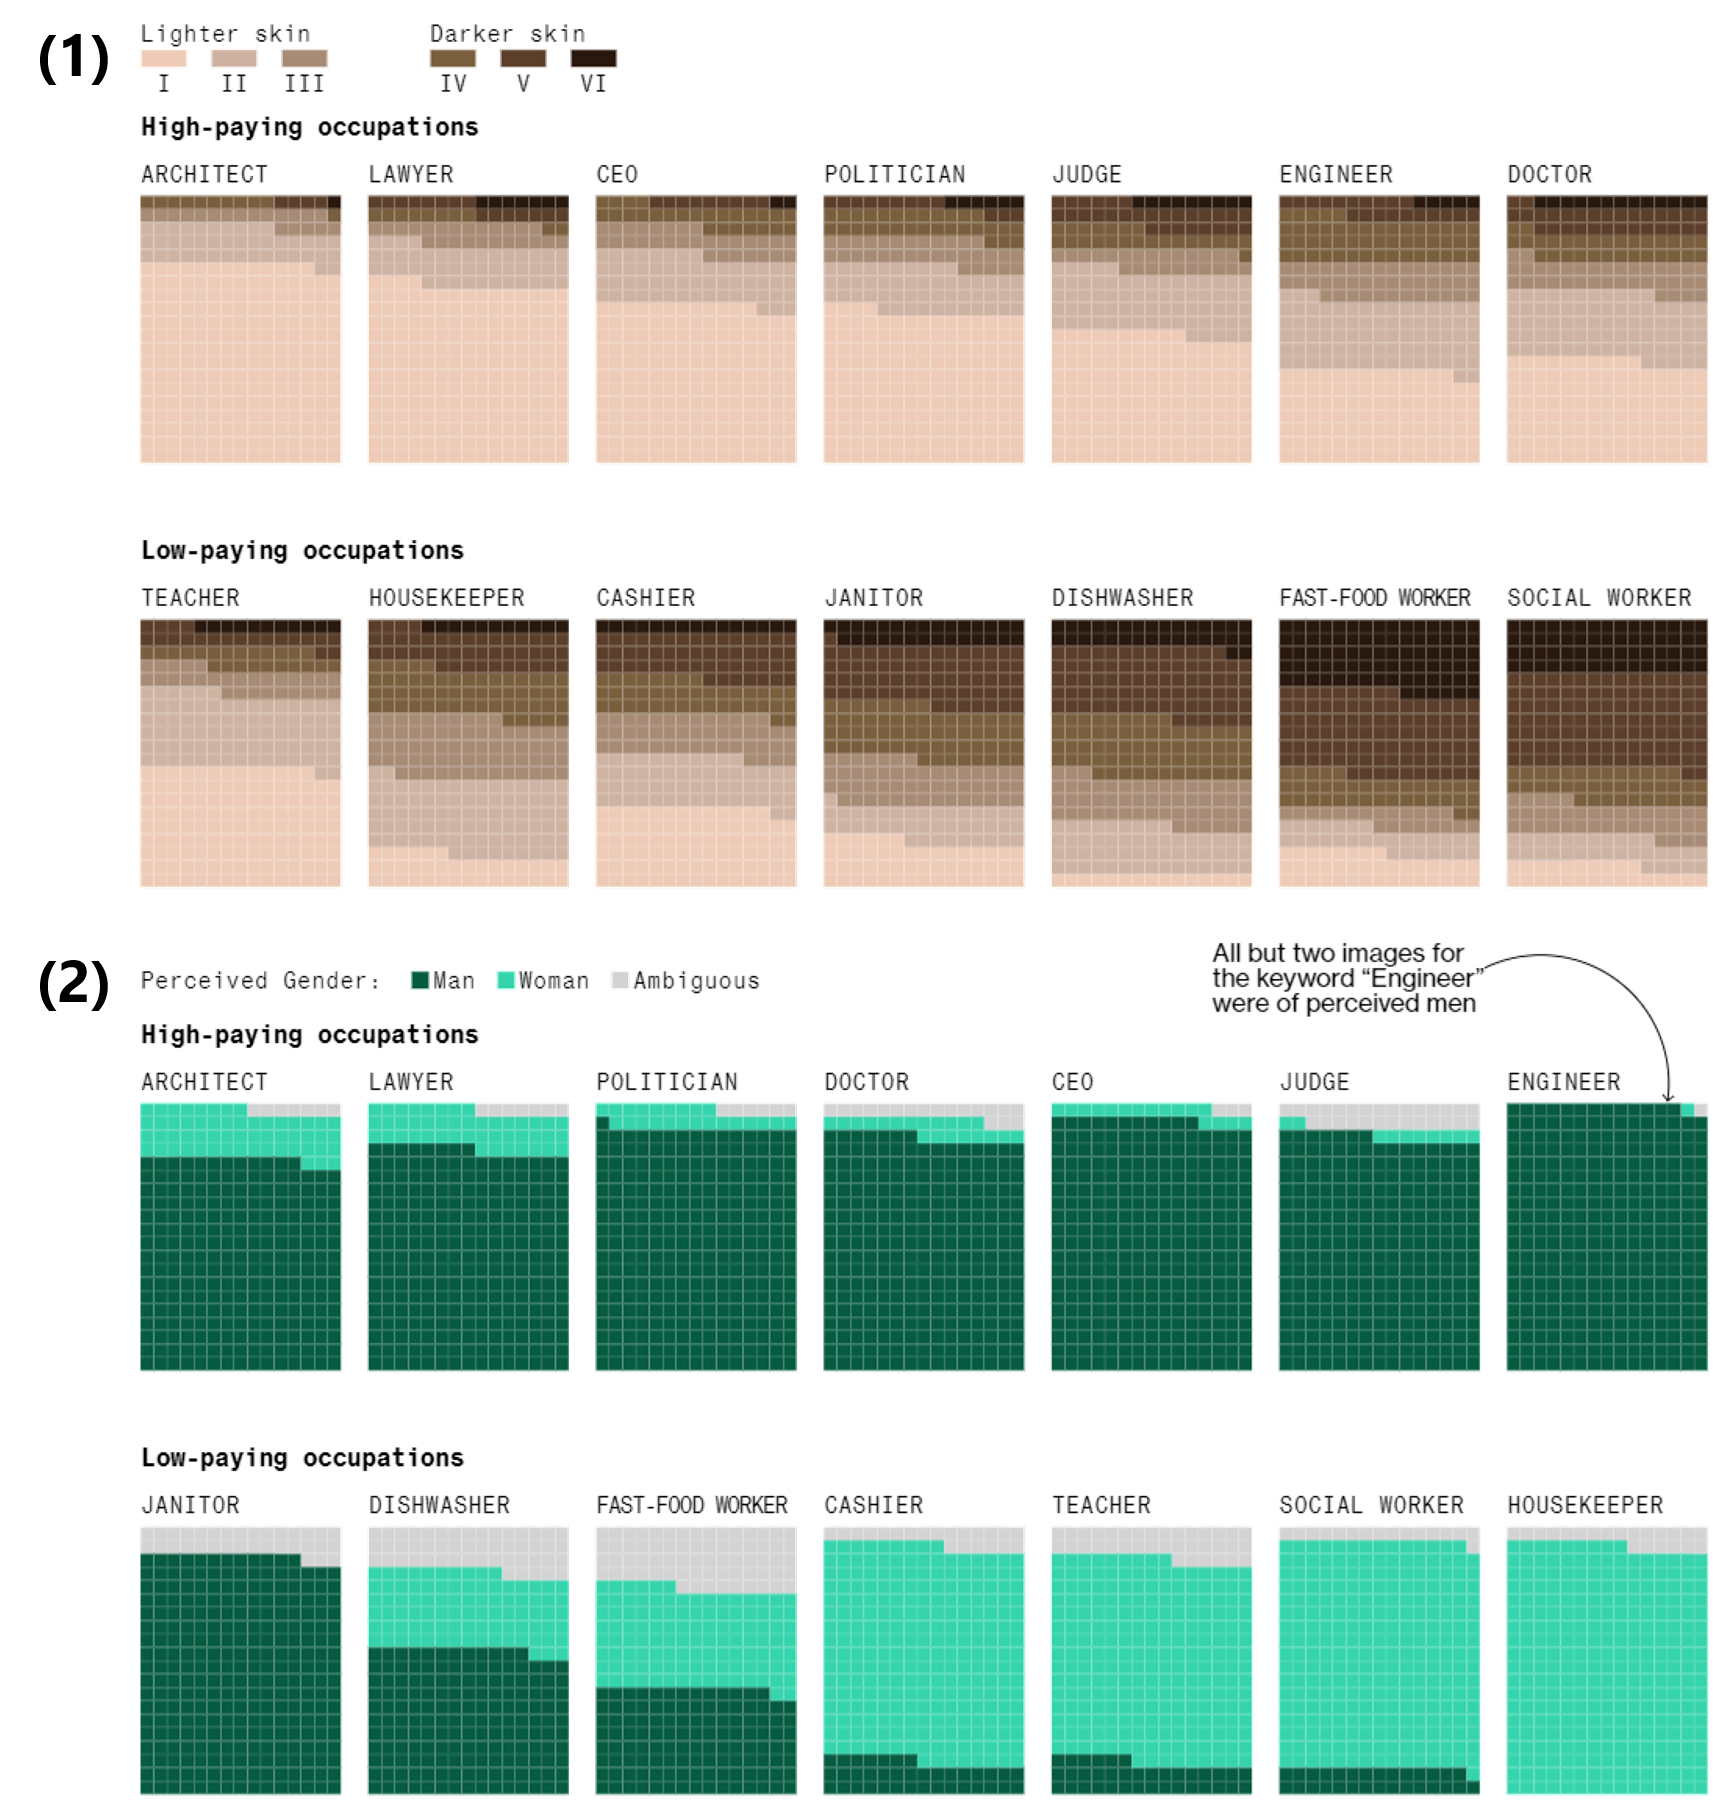
\includegraphics[width=0.75\textwidth]{figures/etatdelart-nicoletti-bass-2023}
					\caption{
						Répartitions des teintes de peaux \textbf{(1)} et des genres \textbf{(2)} par métier lors de génération de portrait avec \texttt{Stable Diffusion} (étude menée par \cite{nicoletti-bass:2023:generative-ai-takes}).
					}
					\label{figure:2.3.1.A-DEFIS-ANNOTATION-ASPECT-DONNEES-REPRESENTATIVITE-STEREOTYPES}
				\end{figure}
				Ici, ce modèle dépeint les inégalités de notre société en perpétuant des stéréotypes, et cela ouvre la question suivante : veut-on vraiment reproduire à l'identique cette représentation ?
				% Exemple pour faire réagir (non utilisé) : Si on veut générer une nouvelle BD Lucky Luke à partir des anciennes BDs, veut-on vraiment encore avoir un chinois à la blanchisserie ?
			\end{leftBarExamples}
			%
			\begin{leftBarIdea}
				% Solution: Équilibrage par la génération de données.
				Une piste pour équilibrer efficacement les corpus d'entraînement et permettre de corriger leurs biais consiste à utiliser des \textbf{données synthétiques} (\cite{jaipuria-etal:2020:deflating-dataset-bias}).
				Ces données peuvent être créées manuellement ou être générées automatiquement (voir \cite{shorten-etal:2021:text-data-augmentation} pour une revue de génération de textes et \cite{shorten-khoshgoftaar:2019:survey-image-data} pour la génération d'image).
				Bien entendue, une telle approche doit restée réfléchie pour ne pas introduire davantage de biais et pour répondre à un objectif précis d'équilibrage du jeu de données.
			\end{leftBarIdea}
			
			% Problème d'obsolescence des données.
			Une dernière difficulté concerne l'\textbf{obsolescence} des données au cours du temps.
			En effet, peu de phénomènes sont immuables, et il est courant de devoir questionner la représentativité d'un problème pour prendre en compte des nouveaux aspects ou corriger des caractéristiques devenues inexactes.
			%
			\begin{leftBarExamples}
				% Exemple de l'estimation du prix d'une BD.
				Ce problème est particulièrement impactant si nous voulons estimer le prix d'une bande dessinée (voir \textsc{Section~\ref{section:2.1.2.A-PRESENTATION-ANNOTATION-EXEMPLES-REGRESSION}}) car les oeuvres vont gagner ou perdre de la valeur avec le temps.
				Par exemple, en $1949$, le premier album de \texttt{Lucky Luke} devait s'acheter pour quelques francs, alors qu'aujourd'hui, cette édition est estimée à plusieurs milliers d'euros.
				
				% Exemple de l'évolution du langage.
				De manière similaire, le traitement du langage constate aussi des évolutions au cours du temps (\textit{nouveaux mots de vocabulaire, nouvelles expressions, influence de langues étrangères, ...}), imposant ainsi la mise à jour des jeux de données.
			\end{leftBarExamples}
		
		
		%%% 2.3.1.B. Problèmes de bruits.
		\subsubsection{Problèmes de bruits}
		\label{section:2.3.1.B-DEFIS-ANNOTATION-ASPECT-DONNEES-BRUITS}
		
			% Introduction : données bruités.
			La qualité d'une base d'apprentissage dépend fortement du bruit qu'elle contient.
			Ce bruit est inévitablement inséré lors de la collecte :
			d'une part, la méthode de collecte elle-même peut en introduire (\textit{instrument de mesure faillible, erreur humaine, ...}) ;
			d'autre part, par soucis de représentativité, le bruit intrinsèque du phénomène va être capturé (\textit{forte variabilité, présence d'irrégularité, ...}).
			Un échantillon de données va donc forcément devoir se confronter 

			% Classification des types de bruits.
			Nous nous inspirons de \cite{maharana-etal:2022:review-data-preprocessing} et de \cite{alasadi-bhaya:2017:review-data-preprocessing} pour dresser une liste de problèmes récurrents sur les données suite à une collecte :
			\begin{itemize}
				% Bruit: 1. Données non pertinentes.
				\item présence de \textbf{données non pertinentes} par rapport au cas d'usage :
				une collecte automatique ou aléatoire peut sélectionner des données n'ayant pas ou peu de rapport avec le phénomène à modéliser.
				Garder de telles données peut introduire de la confusion dans le modèle à entraîner ;
				% Bruit: 2. Variations parasites.
				\item dégradation des données par des \textbf{variations parasites} :
				comme décrit en introduction de cette partie, les bruits peuvent être intrinsèques au phénomène ou être introduits par la méthode de collecte.
				Il convient de lisser ou limiter ces bruits pour ne pas perturber le modèle ;
				% Bruit: 3. Absence de valeurs.
				\item \textbf{absence de valeurs} descriptives essentielles :
				cette absence peut venir d'une erreur de mesure, d'une méconnaissance du phénomène à caractériser, ou simplement d'un oubli.
				Cependant, un trou de description peut rendre inutile une donnée si cela concerne une caractéristique importante du phénomène ;
				% Bruit: 4. Incohérences et ambiguïtés.
				\item présence d'\textbf{incohérences} ou d'\textbf{ambiguïté} entre les données :
				les données sont rarement catégoriques et plusieurs interprétations sont parfois possibles (voir la discussion sur la subjectivité en \textsc{Section~\ref{section:2.3.3.A-DEFIS-ANNOTATION-ASPECT-HUMAIN-INTER-ANNOTATEURS}}).
				Toutefois, des contradictions entre les données peuvent pénaliser le modèle à entraîner.
			\end{itemize}
			%
			\begin{leftBarExamples}
				% Problèmes: estimation du prix d'une BD.
				Pour illustrer ces problèmes, considérons la tâche d'estimation du prix d'une bande dessinée (voir \textsc{Section~\ref{section:2.1.2.A-PRESENTATION-ANNOTATION-EXEMPLES-REGRESSION}}) :
				\begin{itemize}
					% Exemple: 1. Données non pertinentes.
					\item une donnée concernant le prix d'un roman ou d'une encyclopédie avoir été inséré par mégarde et pourrait être considéré comme données non pertinentes pour ce cas d'usage ;
					% Exemple: 2. Variations parasites.
					\item un changement de typographie (\textit{majuscules, minuscules, accents, ponctuation}) dans l'écriture d'un titre pourrait mal identifier une bande dessinée ;
					% Exemple: 3. Absence de valeurs.
					\item une information peut ne pas avoir été renseigné lors d'une transaction (l'année d'édition par exemple), alors que c'est une caractéristique importante de la prise de décision ;
					% Exemple: 4. Incohérences et ambiguïtés.
					\item une même bande dessinée (avec les mêmes caractéristiques) peut avoir été vendue à deux prix radicalement différent, introduisant ainsi une légère ambiguïté dans les données.
				\end{itemize}
				
				% Autres problèmes.
				Des problèmes similaires peuvent impacter le traitement du texte (\textit{fautes de grammaticales ou syntaxiques, ambiguïtés ou sémantiques, omissions, ...}), des images (\textit{flous, mauvais cadrages, colorimétries gênantes, ...}) et de l'audio (\textit{bruits en arrière plan, saturations, coupures inopportunes, ...}).
				% Problème d'image flou: classification de l'état d'une BD.
				Par exemple, dans la tâche de classification de l'état d'une bande dessinée à partir d'une photo (voir \textsc{Section~\ref{section:2.1.2.B-PRESENTATION-ANNOTATION-EXEMPLES-CLASSIFICATION}}), comment juger correctement de l'état d'une \texttt{BD} si la photo capturée est flou ?
			\end{leftBarExamples}
			\todo{prendre des photos en mauvaises qualités de mes BD : flous, main sur l'image, mauvais cadrage, peluche ?}
			
			% Correction des données par le prétraitement et le nettoyage.
			Pour limiter l'impact du bruit dans les données, \cite{alasadi-bhaya:2017:review-data-preprocessing} structurent les étapes de prétraitement de données entre quatre catégories :
			\begin{itemize}
				% Approche: Data cleaning.
				\item le \textbf{nettoyage des données} : cette étape consiste à compléter les données manquantes (\textit{en prenant la valeur moyenne par exemple}), à filtrer les données aberrantes ou inintéressantes, et surtout à lisser le bruit dans les données en gommant les variations parasites ;
				% Approche: Data integration.
				\item l'\textbf{intégration des données} : dans certains cas, plusieurs sources de données sont disponibles, il peut être donc intéressant de croiser ces sources de données pour augmenter la consistance de la base d'apprentissage et identifier les incohérences ;
				% Approche: Data transformation.
				\item le \textbf{formatage des données} : pour exploiter facilement les données, certaines transformations sont parfois nécessaires pour limiter les ambiguïtés dues au leur format (\textit{par exemple: normaliser une valeur entre $0$ et $1$, limiter les caractères spéciaux dans un texte});
				% Approche: Data reduction.
				\item la \textbf{réduction des données} : en réalisant une analyse approfondie des données, on peut quelques fois constater que certaines caractéristiques présentes sur les données sont peu utiles et peuvent être supprimer pour réduire la complexité de la base d'apprentissage.
			\end{itemize}
			\cite{baledent:2022:complexite-annotation-manuelle} rappelle néanmoins que le document source (ou ici : la donnée brute) doit rester accessible pour la phase d'annotation pour ne pas manquer d'information potentiellement intéressante.
			%
			\begin{leftBarExamples}
				% Correction: estimation du prix d'une BD.
				Reprenons les problèmes évoqués précédemment sur la tâche d'estimation du prix d'une bande dessinée :
				\begin{itemize}
					% Correction: 1. Données non pertinentes.
					\item une donnée inintéressante peut simplement être supprimée ;
					% Correction: 2. Variations parasites.
					\item normaliser les champs décrivant une bande dessinée en passant tout en minuscules limiterait les chances de mal l'identifier ;
					% Correction: 3. Absence de valeurs.
					\item une année d'édition manquante pourrait être identifiée par l'étiquette \texttt{inconnue} et un prix manquant pourrait être complété par la moyenne du prix des \texttt{BD} ayant les mêmes caractéristiques ;
					% Correction: 4. Incohérences et ambiguïtés
					\item une prix faussé pourrait être identifié comme incohérent en analysant les prix des \texttt{BD} ayant les mêmes caractéristiques ;
				\end{itemize}
			\end{leftBarExamples}
		
		
		%%% 2.3.1.C. Problèmes d'exploitation et de diffusion.
		\subsubsection{Problèmes d'exploitation et de diffusion}
		\label{section:2.3.1.C-DEFIS-ANNOTATION-ASPECT-DONNEES-DROITS}
		
			% Introduction: toutes les données ne sont pas disponibles.
			En plus des difficultés techniques sur la réalisation d'une collecte de données, il y a aussi contraintes législatives et stratégiques à prendre en compte.
			
			% Contraintes sur la propriété intellectuelle des données.
			D'une part, il faut considérer le fait que certaines données sont protégées et ne peuvent pas être collectées ou exploitées librement.
			C'est le cas de données soumises aux droits de \textbf{propriétés intellectuelles} qui empêchent cet usage : on peut citer par exemple \cite{loignon:2023:ia-medias-francais} qui évoque le levé de bouclier des médias français contre l'utilisation de leur article pour entraîner des modèles de langues, mais aussi \cite{les-echos:2023:ia-auteur-game} qui questionne la violation du \textbf{droit d'auteur} lorsque qu'un modèle est entraîné sur l'oeuvre d'un artiste et qu'il est capable de la reproduire.
			
			% Contraintes sur le consentement.
			Ces limites concernent aussi la Réglementation Générale européenne sur la Protection des Données (\texttt{RGPD}, \cite{european-commission:2016:regulation-eu-2016}) restreignant les \textbf{collectes et usages non consenties} de données personnelles.
			Ainsi, il n'est pas possible d’entraîner n'importe quel modèle sur n'importe quelles données, et une telle contrainte impose de manipuler les données en garantissant l'anonymat et la confidentialité des personnes consentantes.
			
			% Exemple 1 : propriété intellectuelle et consentement.
			\begin{leftBarExamples}
				Considérons la conception d'un modèle de synthèse vocale pour réaliser une audio-\texttt{BD} (voir \textsc{Section~\ref{section:2.1.2.D-PRESENTATION-ANNOTATION-EXEMPLES-TRANSCRIPTION}}).
				D'une part, un tel projet nécessiterait déjà de demander les droits d'adaptation pour entrainer un modèle de synthèse vocale avec les doublage de l'adaptation télévisée de \texttt{Lucky Luke}.
				D'autre part, l'utilisation de la voix d'une personne se confrontera probablement à plusieurs restrictions pour éviter que ce modèle ne soit détourné pour des usages non consentis par le doubleur.
			\end{leftBarExamples}
			
			% Contraintes stratégiques.
			Pour aller plus loin, cette notion de confidentialité touche les données personnelles, mais aussi le \textbf{caractère stratégique} d'une organisation.
			En effet, dans le monde académique, les données manipulées sont le plus souvent publiques et peuvent être employées pour contribuer à la recherche scientifique.
			Mais dans le secteur industriel, les jeux de données sont liés au domaine d'activité de l'entreprise : ils ont généralement requis un investissement conséquent en temps et en moyens, et ils représentent donc son avantage concurrentiel (\textit{par leur spécificité, leur caractère secret ou novateur, leur qualité compétitive, ...}).
			Il est donc rare de voir une entreprise partager ses jeux de données car elle pourrait perdre un de ses atouts stratégiques.
			
			% Exemple OpenSource, mais limitation commerciale.
			Un solution est de ce tourner les jeu de données \textbf{accessibles en \textit{Open Source}}.
			Plusieurs plateformes mettre en effet à disposition des données ou des modèles, comme \textit{Hugging Face} (\cite{hugging-face:2016:hugging-face-ai}) ou \texttt{Zenodo} (\cite{re3data.org:2013:zenodo}).
			Toutefois, deux limites subsistent à l'usage de ces données :
			\begin{itemize}
				\item les données mises à dispositions publiquement sont souvent assez générales et ne reflète pas la spécificité des cas d'usage de l'entreprise, limitant ainsi leur intérêt ;
				\item les données publiques ne sont pas forcément ouvertes à un usage commercial (\textit{elles peuvent par exemple employé la licence \texttt{CC BY-NC 4.0}, \cite{creative-commons:2013:cc-bync-legal}}), restreignant ainsi les seules applications au domaine de la recherche et veille scientifique.
			\end{itemize}
			Pour ne pas faire de faux pas juridique, \cite{rajbahadur-etal:2022:can-use-this} propose une approche pour vérifier si une licence permet d'exploiter un jeu de données.
			
			% Besoin de tracabilité.
			\begin{leftBarInformation}
				Pour terminer nous mentionnons aussi une proposition de législation européenne concernant la futures réglementation des modèles d'intelligence artificielle (\texttt{IA Act}, \cite{european-commission:2021:proposal-regulation-european}).
				Cette loi concerne les quatre objectifs suivants :
				\begin{itemize}
					\item \textguillemets{veiller à ce que les systèmes d'\texttt{IA} mis sur le marché de l'Union et utilisés soient sûrs et respectent la législation en vigueur en matière de droits fondamentaux et les valeurs de l'Union} ;
					\item \textguillemets{garantir la sécurité juridique pour faciliter les investissements et l'innovation dans le domaine de l'\texttt{IA}} ;
					\item \textguillemets{renforcer la gouvernance et l'application effective de la législation existante en matière de droits fondamentaux et des exigences de sécurité applicables aux systèmes d'\texttt{IA}} ;
					\item \textguillemets{faciliter le développement d'un marché unique pour des applications d'\texttt{IA} légales, sûres et dignes de confiance, et empêcher la fragmentation du marché}.
				\end{itemize}
				Un besoin de traçabilité des données et des modèles se fait donc sentir, renforçant les recommandations à documenter et détailler les traitement et choix pour garantir la représentativité et la qualité des données des bases d'apprentissage.
			\end{leftBarInformation}
		
		
	%%%
	%%% Subsection 2.3.2: Défis concernant la complexité inhérente à la tâche d'annotation.
	%%%
	\subsection{Défis concernant la complexité inhérente à la tâche d'annotation}
	\label{section:2.3.2-DEFIS-ANNOTATION-ASPECT-COMPLEXITE}
	
		% Introduction: Se rendre compte de la complexité.
		Selon \cite{baledent:2022:complexite-annotation-manuelle}, deux types de complexités sont à différencier :
		\begin{itemize}
			% Complexité propre aux données.
			\item la \textbf{complexité propre au phénomène} que l'on veut modéliser :
			nous avons pu apercevoir celle-ci dans la \textsc{Section~\ref{section:2.3.1.A-DEFIS-ANNOTATION-ASPECT-DONNEES-REPRESENTATIVITE}}, notamment en considérant la nécessité de collecter une grande quantité de données pour représenter la diversité du phénomène et le besoin de contrôler les bruits pour en assurer la qualité, ...
			% Complexité propre à la procédure d'annotation.
			\item et la \textbf{complexité propre à la procédure d'annotation} mise en place :
			cet aspect est abordée brièvement dans la \textsc{Section~\ref{section:2.2-ORGANISATION-ANNOTATION}} en exposant le besoin d'établir une modélisation du problème avec son guide d'annotation, le recours à un processus itératif pour affiner les problèmes de conception et différences d'interprétation (cycles \texttt{MATTER} et \texttt{MAMA}), ou encore l'intervention de différents utilisateurs ayant des compétences différentes.
		\end{itemize}
		Dans cette section, nous allons voir comment analyser et mesurer cette complexité, puis nous nous intéresserons aux coûts qu'elle peut engendrer lors de la conception du jeu de données.
		
		
		%%% 2.3.2.A. Modélisation difficile du phénomène.
		\subsubsection{Modélisation difficile du phénomène}
		\label{section:2.3.2.A-DEFIS-ANNOTATION-ASPECT-COMPLEXITE-MODELISATION}
		
			% Introduction : Modélisation importante, mais compliquée !
			Comme nous l'avons énoncé lors de la présentation au cours du cycle \texttt{MATTER} en \textsc{Section~\ref{section:2.2.1.A-ORGANISATION-ANNOTATION-ETAPES-CLES-MODELIZE-ANNOTATE}}, la modélisation est une étape importante du processus de conception car elle permet de clarifier ce qu'il faut annoter et avec quel(s) objectif(s).
			Toutefois, plusieurs aspects rendent cette tâche difficile à réaliser.
			
			% Complexité due à l'intervention d'experts métiers.
			Tout d'abord, le projet d'annotation concerne généralement un cas d'usage précis dont la spécificité requiert l'intervention d'experts ayant des \textbf{connaissances métiers}.
			Cependant, de tels experts n'ont pas forcément les compétences analytiques requises pour établir une représentation abstraite de leurs connaissances.
			En effet, diverses questions sont à discuter concernant la modélisation à choisir :
			\begin{itemize}
				\item quel standard existe-t-il qui soit réutilisable dans ce cas d'usage ?
				\item sera-t-elle stable et explicite à l'annotation ?
				\item sera-t-elle traduite en un seul ou en plusieurs modèle(s) de \textit{Machine Laening} ?
				\item sera-t-elle maintenable avec de grands volumes de données ?
			\end{itemize}
			Pour y répondre, ateliers de conception sont généralement organiser avec les experts, permettant ainsi d'identifier les notions pertinentes à intégrer dans la modélisation finale du problème.
			Si le phénomène est intrinsèquement complexe, il est possible néanmoins que ces ateliers se réalisent en mode essai-erreur (à l'image du mini-cycle \texttt{MAMA}) jusqu'à trouver une modélisation qui puisse convenir, rendant cette tâche particulièrement pénible.
			%
			\begin{leftBarExamples}
				Pour se rendre compte de cette difficulté, essayons par exemple de détailler l'ensemble des actions que peut entreprendre un robot conversationnel en domotique (comme \texttt{Alexa}, \cite{alexa-internet:2018:keyword-research-competitor}), et modélisons ensuite les diverses instructions verbales pouvant déclencher ces actions.
			\end{leftBarExamples}
			
			% Complexité due à la rigueur requise pour la conception.
			Dans un second temps, il est nécessaire de structurer cette modélisation dans le but de \textbf{rédiger le guide d'annotation} associé (voir \textsc{Section~\ref{section:2.2.1.A-ORGANISATION-ANNOTATION-ETAPES-CLES-MODELIZE-ANNOTATE}}).
			\cite{nedellec-etal:2006:annotation-guidelines-machine} a pu montrer que la clarté de ce guide impacte directement la qualité des annotations : il est donc important de rédiger celui-ci avec soin pour donner à l'annotateur une vision de son objectif (\cite{fort-etal:2009:vers-methodologie-annotation}).
			Cela requiert toutefois de solides compétences analytiques et pédagogiques, notamment pour définir, organiser et transmettre ce vaste ensemble des règles sans introduire de biais ni de confusion.
			%
			\begin{leftBarInformation}
				Nous rappelons que \cite{dipper-etal:2004:useradaptive-annotation-guidelines} a dressé une liste de recommandations pour rédiger un guide d'annotation fiable.
			\end{leftBarInformation}
			
			% Complexité due à la subjectivité de la tâche.
			Malgré tout, \cite{baledent:2022:complexite-annotation-manuelle} rappelle que l'établissement d'une modélisation d'un phénomène \textbf{relève d'un choix}, et que celui-ci est par conséquent subjectif.
			En effet, plusieurs représentations peuvent convenir à un même cas d'usage, et celui retenu devra être celui qui correspondra le plus à la finalité de votre modèle.
			Ce choix, aussi avisé soit-il, entrera inévitablement en friction avec certaines données collectées qui s'inséreront difficilement au sein de la modélisation choisie.
			Lors de la rédaction du guide d'annotation, il faut donc trouver l'équilibre entre entre la rigueur (\textit{pour fiabiliser la qualité de la labellisation}) et la flexibilité (\textit{pour pouvoir s'adapter aux données contrariantes}).
			
			% Solution pour limiter la complexité de modélisation.
			\begin{leftBarIdea}
				Quelques pistes approches peuvent être mises en places pour assister la modélisation d'un problème :
				\begin{itemize}
					% Solution: Modélisation non-supervisées (clustering ou topic modelling).
					\item les approches \textbf{non supervisées} :
					elles consistent à laisser la machine extraire et structurer automatiquement la connaissance contenue dans les données collectées.
					Par exemple pour le traitement du texte, nous pouvons citer les méthodes d'exploration utilisant le regroupement automatique (\textit{clustering}) comme KMeans (\cite{macqueen:1967:methods-classification-analysis}), ou la modélisation thématique (\textit{topic modeling}) comme \text{LDA} (\cite{blei-etal:2003:latent-dirichlet-allocation}) ;
					% Solution: Modélisation semi-supervisées (active learning)
					\item les approches \textbf{semi-supervisées} :
					elles consistent à travailler main dans la main avec la machine pour explorer les données collectées.
					On peut citer par exemple les méthodes d'apprentissage actif (\textit{active learning}) dont une revue est proposée par \cite{settles:2010:active-learning-literature} ;
					% Solution: Modélisation itératives.
					\item les approches \textbf{itératives} :
					elles consistent à concevoir d’abord un petit modèle dont le périmètre est limité, puis d'étendre pas à pas son périmètre suite aux retours de son utilisation.
					Une organisation fait bien entendu écho à la philosophie du cycle \texttt{MATTER}.
				\end{itemize}
				Toutefois, plusieurs handicaps pénalisent ces approches, notamment lorsque les données bruitées, déséquilibrées ou dont l'interprétation nécessite une forte connaissance métier.
			\end{leftBarIdea}
			
			% Avis de l'auteur : pas d'assistance à la modélisation !
			\begin{leftBarAuthorOpinion}
				% Constat: conception généralement manuelle et peu assister.
				De part notre expérience, nous constatons que peu d'approches non-supervisés ou semi-supervisées sont utilisées, notamment parce que leur résultats sont jugés peu pertinents sur des phénomènes complexes.
				Les experts métiers réalisent alors cette étape de modélisation manuellement, absorbant la complexité de cette tâche en organisant de nombreux ateliers de conception en mode essai-erreur.
				
				% Exemple des chatbots.
				C'est particulièrement le cas lors de la concevoir de la base d'apprentissage d'un assistant conversationnelle (\textit{task-oriented}) : la tâche de modélisation consiste généralement à identifier l'intention formulée dans une demande utilisateur en fonction du verbe d'action (\textguillemets{\textit{je veux \textbf{réserver} un billet}}, \textguillemets{\textit{\textbf{joue} moi du jazz !}}, \textguillemets{\textit{comment \textbf{éditer} une attestation ?}}).
				Cependant, la vaste diversité du langage permet rarement d'identifier les thématiques présents dans une collecte de données.
				L'étape de modélisation est alors réalisée manuellement par les experts du domaine couvert par l'assistant conversationnel.
			\end{leftBarAuthorOpinion}
		
		%%% 2.3.2.B. Estimation de la complexité.
		\subsubsection{Estimation de la complexité}
		\label{section:2.3.2.B-DEFIS-ANNOTATION-ASPECT-COMPLEXITE-ESTIMATION}
			
			% Estimation par une approche analytique.
			Dans \cite{fort-etal:2012:modeling-complexity-manual} puis dans \cite{fort-etal:2012:modeling-complexity-manual}, une approche analytique est proposée pour mesurer la complexité des tâches de modélisation et d'annotation.
			Six dimensions sont détaillées, réparties en trois axes :
			\begin{itemize}
				% Aspect localisation.
				\item la complexité de \textbf{localisation} de l'annotation (\textit{discrimination}, \textit{délimitation}) :
				y a-t-il plusieurs parties à annoter dans une donnée ?
				quel est le ratio entre les parties à annoter et les parties potentiellement annotables ?
				est-ce que ces parties sont clairement délimitées ou ont-elles des bornes floues ?
				% Aspect caractérisation.
				\item la complexité de \textbf{caractérisation} de l'annotation (\textit{expressivité}, \textit{dimensionnalité}, \textit{ambiguïté}) :
				doit-on annoter une variable catégorielle ou numérique ?
				s'il y a plusieurs variables entre elles, y a-t-il des relations entre elles ?
				leur cardinalité est-elle finie ou infinie ?
				quelle est la proportion de confusion ou de désaccord d'interprétation de cette modélisation ?
				% Aspect contexte.
				\item la complexité de \textbf{situation} de l'annotation (\textit{poids du contexte}) :
				a-t-on besoin d'informations complémentaires pour être capable d'interpréter la donnée ?
			\end{itemize}
			
			% Estimation par une approche statistique.
			Une autre manière de mesurer la complexité d'une tâche d'annotation consiste à \textbf{évaluer les différences entre annotateurs}.
			En effet, \cite{gut-bayerl:2004:measuring-reliability-manual} ont notamment montré qu'un nombre élevé de désaccords de labellisation peut mettre en avant une ambiguïté de modélisation, une différence d'interprétation entre annotateurs, ou encore une difficulté à saisir pleinement la subtilité des données manipulées : dans tous les cas, ces désaccords témoignent de la complexité de la tâche.
			Pour mesurer cet accord, différents scores ont été développés comme peut en témoigner la revue de \cite{artstein-poesio:2008:intercoder-agreement-computational}.
			Nous reviendrons plus en détails sur ces différences de comportement dans la \textsc{Section~\ref{section:2.3.3-DEFIS-ANNOTATION-ASPECT-HUMAIN}}.
			\begin{leftBarInformation}
				L'un des plus scores les plus utilisé est $\alpha$ de \textit{Krippendorff} (\cite{krippendorff:2004:content-analysis-introduction}).
				Le score est normalisé entre $0$ (\textit{aucun accord}) et $1$ (\textit{accord parfait}).
				On considère un accord fort lorsque le score est supérieur à $0.8$,
				et l'accord reste acceptable si la valeur est supérieure à $0.667$.
			\end{leftBarInformation}
			
			% Exemples
			\begin{leftBarExamples}
				% Exemple: Identification d'une bande dessinée à partir de sa couverture.
				Considérons l'identification d'une bande dessinée à partir de sa couverture, pour laquelle l'annotation de textes présents sur une image sont nécessaires pour entraîner un modèle de reconnaissance optique de caractères (voir \textsc{Section~\ref{section:2.1.2.C-PRESENTATION-ANNOTATION-EXEMPLES-EXTRACTION}}).
				Nous pouvons voir que :
				\begin{itemize}
					% Aspect localisation.
					\item la localisation des annotations est assez évidente car l'information est visuelle : 
					(1) En général, il y a peu de textes sur une couverture de \texttt{BD}, l'information est donc facilement identifiable (\textit{bonne discrimination}) ;
					(2) Cependant, il peut y avoir de légères différences sur la position exacte des boxes entourant les textes (\textit{délimitation délicate}) ;
					% Aspect caractérisation.
					\item la caractérisation concerne du texte mais son annotation est explicite :
					(1) L'annotation concerne du texte et des nombres, il y a donc une grande variabilité parmi les valeurs possibles (\textit{forte expressivité}).
					(2) Plusieurs informations sont attendues, comme le nom de la collection, l'auteur, le titre, ou la date de parution (\textit{dimensionnalité modérée}) ;
					(3) Toutefois, il y a assez peu de doute sur les valeurs à indiquer car ces dernières sont explicitement liées aux inscriptions sur l'image (\textit{peu d'ambiguïté}) ;
					% Aspect contexte.
					\item la situation de l'annotation n'a pas d'impact :
					en effet, peu d'informations complémentaires sont requise pour interpréter les textes de l'image (\textit{poids du contexte faible}).
				\end{itemize}
				Au final, l'analyse révèle que cette tâche est relativement peu complexe.
				Le calcul d'un score d'accord entre annotateurs permettrait de confirmer cette hypothèse et d'en déduire la confiance que nous pouvons accordé à la qualité des données labellisées.
			\end{leftBarExamples}
			
			
		%%% 2.3.2.C. Problèmes de coûts.
		\subsubsection{Problèmes de coûts}
		\label{section:2.3.2.C-DEFIS-ANNOTATION-ASPECT-COMPLEXITE-COUTS}
		
			% Introduction : Une conséquence de la complexité est le coût de l'annotation.
			Toute cette complexité a un impact non négligeable sur les coûts à engager dans un projet de conception de jeu de données.
			Nous allons ici détailler certains de ces coûts et donner quelques exemples notoires.
			
			% Coût embauches.
			Tout d'abord, il y a des \textbf{charges de main d'oeuvre}.
			En effet, de nombreuses personnes aux compétences diverses vont s'investir dans un tel projet (voir \textsc{Section\ref{section:2.2.2-ORGANISATION-ANNOTATION-ACTEURS}}), à la fois pour modéliser le phénomène mais aussi pour labelliser les données le représentant.
			L'intervention de ces acteurs va engager des coûts dans l'embauche des experts et opérateurs nécessaires, mais aussi dans leur formation si cela est nécessaire (veille technologique, montée en compétence sur la compréhension du phénomène, ...).
			
			% Coût temporel.
			Ensuite, il faut considérer les \textbf{facteurs temporels} qui impactent le délais de mise en production du modèle de \textit{Machine Learning}.
			En plus des délais de monté en compétences des experts, nous pouvons ajouter :
			\begin{itemize}
				\item le temps nécessaire à la \textit{collecte de données}, pouvant prendre plusieurs semaines celle-ci correspond à un sondage ou à une mesure d'un phénomène s'étalant sur la durée ;
				\item le temps imposé par les \textit{ateliers de conception} de la modélisation, pouvant prendre entre quelques heures et quelques semaines en fonction de sa complexité et des différences d'opinions entre experts ;
				\item le temps dédié à l'\textit{annotation des données}, dépendant entre autre de la complexité de la modélisation et de la quantité à labelliser ;
				\item et le temps requis pour entraîner le modèle de \textit{Machine Learning}.
			\end{itemize}
			A cela s'ajouter aussi la perspective de révision de la modélisation, et donc à la multiplication des coûts en appliquant plusieurs itérations du cycle \texttt{MATTER} pour obtenir un modèle convenable.
			Il est possible de réduire certains de ces coûts temporels en ajoutant davantage de personnes dans le projet, mais cela augmentera évidemment les charges de main d'oeuvre, et quelques aspects demeureront toutefois incompressibles (les débats lors de la phase de modélisation par exemple).
			
			% Coût financiers.
			Enfin, il y a divers \textbf{coût financiers à engager} en plus des recrutements et des conséquences des délais de réalisation.
			On peut notamment considérer l'infrastructure technique tel que l'outil d'annotation et de stockage des données, les potentiels instruments de mesure du phénomène (micro, caméra, sondes, ...) ou encore les acquisition de droits d'utilisations de données ou de modèles sous licence.
			
			% Exemple de coûts.
			\begin{leftBarExamples}
				Détaillons ici deux projets d'annotation dont le chiffrage est disponible :
				\begin{itemize}
					% Prague Dependency Treebank.
					\item \texttt{Prague Dependency Treebank} (\cite{bohmova-etal:2003:prague-dependency-treebank}): L'annotation de $180~000$ phrases tchèques (environ $1.8$ million de \textit{tokens}) pour l'analyse morpho-syntaxique a duré $5$ ans (entre 1996 et 2003), impliquant $22$ personnes. La somme totale engagée est estimée à $600~000$ dollars ;
					% MS COCO.
					\item \texttt{MS COCO} \cite{lin-etal:2014:microsoft-coco-common}: L’annotation d'objets présent dans $328~000$ images (environ $2.5$ millions d'objet de $91$ types différents) a nécessité environ $70~000$ d'annotation.
				\end{itemize}
			\end{leftBarExamples}
			
			% Solutions pour limiter les coûts
			\begin{leftBarIdea}
				Pour limiter les coûts, diverses solutions ont déjà été proposées :
				\begin{itemize}
					% Solution: Pré-annotation pour préparer le travail de l'annotateur.
					\item la \textbf{pré-annotation} :
						cette approche consiste à employer un petit modèle pour suggérer une annotation à l'annotateur, celui-ci pouvant alors l'approuver ou corriger.
						\cite{fort-sagot:2010:influence-preannotation-postagged} démontre le gain de temps et de qualité d'une telle approche.
						toutefois, certains biais peuvent influence négativement l'annotateur : \cite{dandapat-etal:2009:complex-linguistic-annotation} souligne par exemple le risque de biais de confirmation (influence de la machine et tendance de l'annotateur d'être en accord avec celle-ci, notamment sur des données ambiguës) ;
					% Solution: Apprentissage actif pour cibler le travail de l'annotateur.
					\item l'\textbf{apprentissage actif} (\textit{active learning}) :
						cette approche consiste à interagir avec la machine pour sélectionner les données les plus intéressantes à annoter (\cite{settles:2010:active-learning-literature}).
						On peut par exemple entraîner un modèle avec les données déjà disponibles, le tester sur les données non annotés et sélectionner les données sur lesquelles ses prédictions sont le moins confiantes ;
					% Solution: Transfert d'apprentissage pour demander moins de données annotées.
					\item le \textbf{transfert d'apprentissage} (\textit{transfert learning}) :
						cette approche consiste à réutiliser la connaissance contenue dans un modèle déjà existant dans le but d'exploiter certaines de ces fonctionnalités (\cite{zhuang-etal:2021:comprehensive-survey-transfer}, \cite{iman-etal:2023:review-deep-transfer}).
						Il a été montré qu'adapter un modèle pour un nouveau cas d'usage similaire peut se faire avec peu de données, réduisant ainsi drastiquement la charge d'annotation (\cite{parnami-lee:2022:learning-few-examples}) ;
					% Solution: Myriadisation.
					\item la \textbf{myriadisation} (\textit{crowdsourcing}) :
						cette approche consiste à déléguer l'annotation à des plateformes collaboratives en ligne comme \texttt{Amazon Mechanical Turk} (\cite{callison-burch-dredze:2010:creating-speech-language}) ou \texttt{Language ARC} (\cite{fiumara-etal:2020:languagearc-developing-language}).
						N'importe quel internaute peut alors contribuer à la tâche d'annotation, permettant ainsi de labelliser de grand volume de données rapidement et à moindre coûts.
						Ces techniques comporte toutefois un inconvénient majeur : les opérateurs ne sont généralement pas des experts et sont rémunérés au volume labellisé.
						La qualité des annotations risque donc d'être délaissée au profit de la quantité.
				\end{itemize}
			\end{leftBarIdea}
		
		
	%%%
	%%% Subsection 2.3.3: Défis concernant les différences de comportements d'annotation.
	%%%
	\subsection{Défis concernant les différences de comportements d'annotation}
	\label{section:2.3.3-DEFIS-ANNOTATION-ASPECT-HUMAIN}
		
		% Introduction: Considérer les différences de comportements.
		On peut constater deux divergences de comportements :
		\begin{itemize}
			\item ceux entre deux annotateurs (voir \textsc{Section~\ref{section:2.3.3.A-DEFIS-ANNOTATION-ASPECT-HUMAIN-INTER-ANNOTATEURS}}) ;
			\item ceux d'un annotateur avec lui-même (voir \textsc{Section~\ref{section:2.3.3.B-DEFIS-ANNOTATION-ASPECT-HUMAIN-INTRA-ANNOTATEURS}}).
		\end{itemize}
		
		
		%%% 2.3.3.A. Différences inter-annotateurs.
		\subsubsection{Différences inter-annotateurs}
		\label{section:2.3.3.A-DEFIS-ANNOTATION-ASPECT-HUMAIN-INTER-ANNOTATEURS}
		
			% Introduction : l'annotation est subjective.
			Comme nous avons pu le voir dans la \textsc{Section~\ref{section:2.3.2.A-DEFIS-ANNOTATION-ASPECT-COMPLEXITE-MODELISATION}}, la modélisation d'un phénomène relève d'un choix subjectif.
			Il est donc normal de constater que cette subjectivité entraîne des différences de comportement d'annotation.
			Celles-ci se manifestent particulièrement sur des données ambiguës ou bruitées car les limites de la modélisation sont exposées.
			D'autres éléments comme le caractère abstrait d'une modélisation ou la présence de règles de labellisation trop floues peuvent aussi mener à des divergences d'interprétation entre opérateurs.
			
			% Facteur de désaccords.
			\cite{bayerl-paul:2011:what-determines-intercoder} ont pu étudier un ensemble de \textbf{facteurs source de désaccords}. Nous en dressons une liste résumée ci-dessous :
			\begin{itemize}
				% Complexité.
				\item la \textit{complexité} du problème :
				que celle-ci vienne intrinsèquement du phénomène à annoter ou du cas d'usage reflétée dans la modélisation, on constate si l'annotation est difficile, alors les chances d'interpréter différemment les données est plus élevée ;
				% Nombre.
				\item le \textit{nombre} d'annotateurs :
				il est normal de constater que plus y a de personnes donnant leurs avis, les avis peuvent diverger ;
				% Expertise.
				\item le \textit{niveau d'expertise} des annotateurs :
				on constate des divergences d'opinion entre les opérateurs agnostique du phénomène et ceux détenant des connaissances sur celui-ci (un linguiste pour des données textuelles, un libraire pour des \texttt{BD}, ...), on constate alors des différences entre
				% Formation.
				\item le \textit{niveau de formation} des annotateurs :
				on constate des divergences de labellisation entre les opérateurs formés à l'outil et au guide d'annotation et ceux découvrant la tâche d'annotation et sa mise en oeuvre pour la première fois.
			\end{itemize}
			%
			\begin{leftBarInformation}
				\cite{bayerl-paul:2011:what-determines-intercoder} montrent aussi qu'il peuvent y avoir des différences entre deux annotateurs experts non-formés, alors qu'il y a moins de divergences entre des annotateurs expert et non-expert s'ils sont formés tous les deux.
				Cela souligne bien l'\textbf{importance de la formation à la tâche d'annotation} et la nécessité de rédiger un guide d'annotation qui détaille l'objectif et les règles de labellisation dans le but d'en limiter la subjectivité.
			\end{leftBarInformation}
			%
			\begin{leftBarIdea}
				% Besoin de formation.
				Comme nous l'avons vu, \cite{bayerl-paul:2011:what-determines-intercoder} recommande de \textbf{simplifier la modélisation} à appliquer et de \textbf{former les opérateurs} à la tâche d'annotation.
				
				% Adjudication.
				Pour aller plus loin, il est recommandé d'organiser des sessions d'\textbf{adjudication} durant laquelle les opérateurs confronter leurs visions en annoter les mêmes données.
				Cela permettra de mesurer un score d'accord entre annotateurs et de discuter des points de désaccords dans l'application du guide de labellisation.
				Une règle de bon sens consiste à confronter $2$ annotateurs pour être capable d'identifier ces points de désaccords, mais il faut être au moins $3$ pour les résoudre.
				\cite{bayerl-paul:2011:what-determines-intercoder} conseille d'ailleurs d'être au moins $5$ annotateurs si le cas d'usage est critique.
			\end{leftBarIdea}
		
		%%% 2.3.3.B. Différences intra-annotateurs.
		\subsubsection{Différences intra-annotateurs}
		\label{section:2.3.3.B-DEFIS-ANNOTATION-ASPECT-HUMAIN-INTRA-ANNOTATEURS}
		
			\todo[inline]{régulation charge de travail}
				% Constat: Erreurs d'inattention, aléas du quotidien
				% Explication: Régulation de la charge de travail: \cite{sperandio:1987:ergonomie-travail-mental}, \cite{sperandio:1972:charge-travail-regulation}, \cite{sperandio:1978:regulation-working-methods}: La tache est perçu comme compliquée, et mes capacités sont perçues comme "minimes" ; Donc l'opérateur va toujours s'adapter pour avoir une complexité "acceptable". Conclusion : j'adapte mes règles d'annotation pour avoir une charge "perçu" plus faible.
			\todo[inline]{quelques solutions: guide, revues, limiter le changement de contexte, gamification}
				% faire une petite partie est parfois plus efficace, mais ne permet pas toujours de résoudre le problème dans sa globalité (on n'a pas l'objectif final)
				% > [fort-etal:2012:modeling-complexity-manual] trop de contexte induit de la complexité
			
			% Dérives.
			\todo[inline]{travail mal reconnu voire ingrat}
				% \cite{valette:2016:analyse-statistique-donneesa} critique le TALN où l'expert linguiste est devenu un vulgaire soustraitant...
				% \cite{perrigo-zorthian:2023:exclusive-openai-used}: Polémique OpenAI sur l'annotation par des Kényan à bas coûts \\
				% \cite{dzieza:2023:ai-lot-work} Payé pour 3 fois rien, une sous classe de travail mal payé émerge
			\todo[inline]{troubles}
				% \cite{rowe:2023:it-destroyed-me}: modérateurs de contenus offensant
	
	%%%
	%%% Conclusion.
	%%%
	\begin{leftBarSummary}
		\begin{todolist}
			\item[\itemok] L'enjeu d'un projet d'annotation consiste à avoir des \textbf{données de qualité} qui soient représentatives du problème à traiter ;
			\item[\itemok] Or la tâche d'annotation et son exigence de qualité engendre de la \textbf{complexité}, et donc une \textbf{charge de travail élevée} ;
			\item[\itemok] Pour réguler cette charge de travail élevée, chaque opérateur va \textbf{adapter sa tâche} pour la rendre supportable, créant alors des \textbf{différences de comportement}.
		\end{todolist}
	\end{leftBarSummary}